\documentclass[11pt]{article}
\usepackage[utf8]{inputenc}

%%% PAGE DIMENSIONS
\usepackage{geometry}
\geometry{a4paper}

\usepackage{graphicx}

%%% PACKAGES
\usepackage{booktabs}
\usepackage{paralist}
\usepackage{verbatim}
\usepackage{subfig}
\usepackage{chngcntr}
\usepackage{tikz}
\usepackage[colorlinks = true,
            linkcolor = black,
            urlcolor  = blue,
            citecolor = blue,
            anchorcolor = blue]{hyperref}
\usepackage[spanish]{cleveref}
\usepackage{placeins}
\usepackage{float}

%%% HEADERS & FOOTERS
\usepackage{fancyhdr}
\pagestyle{fancy}
\renewcommand{\headrulewidth}{0pt}
\lhead{}\chead{}\rhead{}
\lfoot{}\cfoot{\thepage}\rfoot{}

%%% SECTION TITLE APPEARANCE
\usepackage{sectsty}
\allsectionsfont{\sffamily\mdseries\upshape}

%%% ToC (table of contents) APPEARANCE
\usepackage[nottoc,notlof,notlot]{tocbibind} % Put the bibliography in the ToC
\usepackage[titles,subfigure]{tocloft} % Alter the style of the Table of Contents
\renewcommand{\cftsecfont}{\rmfamily\mdseries\upshape}
\renewcommand{\cftsecpagefont}{\rmfamily\mdseries\upshape} % No bold!


\graphicspath{ {images/} }

\counterwithin*{figure}{section}
\counterwithin*{figure}{subsection}
\counterwithin*{figure}{subsubsection}

\counterwithin*{table}{section}
\counterwithin*{table}{subsection}
\counterwithin*{table}{subsubsection}

\addtolength{\cftfignumwidth}{2em}

\renewcommand{\thefigure}{
  \ifnum\value{subsection}=0
    \thesection.\arabic{figure}
  \else
    \ifnum\value{subsubsection}=0
      \thesubsection.\arabic{figure}
    \else
      \thesubsubsection.\arabic{figure}
    \fi
  \fi
}

\renewcommand{\thetable}{
  \ifnum\value{subsection}=0
    \thesection.\arabic{table}
  \else
    \ifnum\value{subsubsection}=0
      \thesubsection.\arabic{table}
    \else
      \thesubsubsection.\arabic{table}
    \fi
  \fi
}

%%% END Article customizations

%%% The "real" document content comes below...

\title{\Large Seguridad en Redes\\Practica 3.3}
\author{David Antuña Rodríguez\\Javier Carrión García}
\date{}

\begin{document}
  \raggedright

  \maketitle
  \newpage

  \section{Filtrado de paquetes}
    \subsection{Reglas para servidores externos}
      \begin{itemize}
        \item Aceptar paquetes reenviados recibidos por la interfaz interno
          (eth1)\\
          \vspace{2mm}
          sudo iptables -A FORWARD -i eth1 -j ACCEPT
        \item Aceptar paquetes reenviados recibidos por la interfaz externo
          (eth2) con el puerto destino HTTP o SSH y la dirección IP destino de
          interno.\\
          \vspace{2mm}
          sudo iptables -A FORWARD -i eth2 -p tcp --dport 22 -d 192.168.1.2 -j
            ACCEPT\\
          sudo iptables -A FORWARD -i eth2 -p tcp --dport 80 -d 192.168.1.2 -j
            ACCEPT
        \item Aceptar paquetes reenviados recibidos por la interfaz externo
          pertenecientes a conexiones establecidas y relacionadas.\\
          \vspace{2mm}
          sudo iptables -A FORWARD -i eth2 -m state --state ESTABLISHED,RELATED
            -j ACCEPT\\
        \item Registrar (LOG) el resto de paquetes reenviados (que serán
          descartados). Los paquetes descartados quedarán registrados en el
          fichero /var/log/syslog.\\
          \vspace{2mm}
          sudo iptables -N LOGGING\\
          sudo iptables -A FORWARD -j LOGGING\\
          sudo iptables -A LOGGING -m limit --limit 2/min -j LOG --log-prefix
            "Dropped:" --log-level 4\\
          sudo iptables -A LOGGING -j DROP
      \end{itemize}

      \par
      \textbf{¿Se puede hacer el ping desde las dos máquinas?}\\
      No, solo desde interno porque aceptamos nuevas conexiones de eth1 en el
      router y no de eth2. El ping sigue funcionando porque hay un funcionando
      porque hay una regla que permite conexiones si el estado es established o
      related.

      \bigskip
      \par
      \textbf{¿Se pueden hacer las conexiones HTTP y SSH a las dos máquinas?}\\
      Tanto en HTTP como en SSH funcionan las conexiones en ambos sentidos.

      \begin{figure}[H]
        \centering
        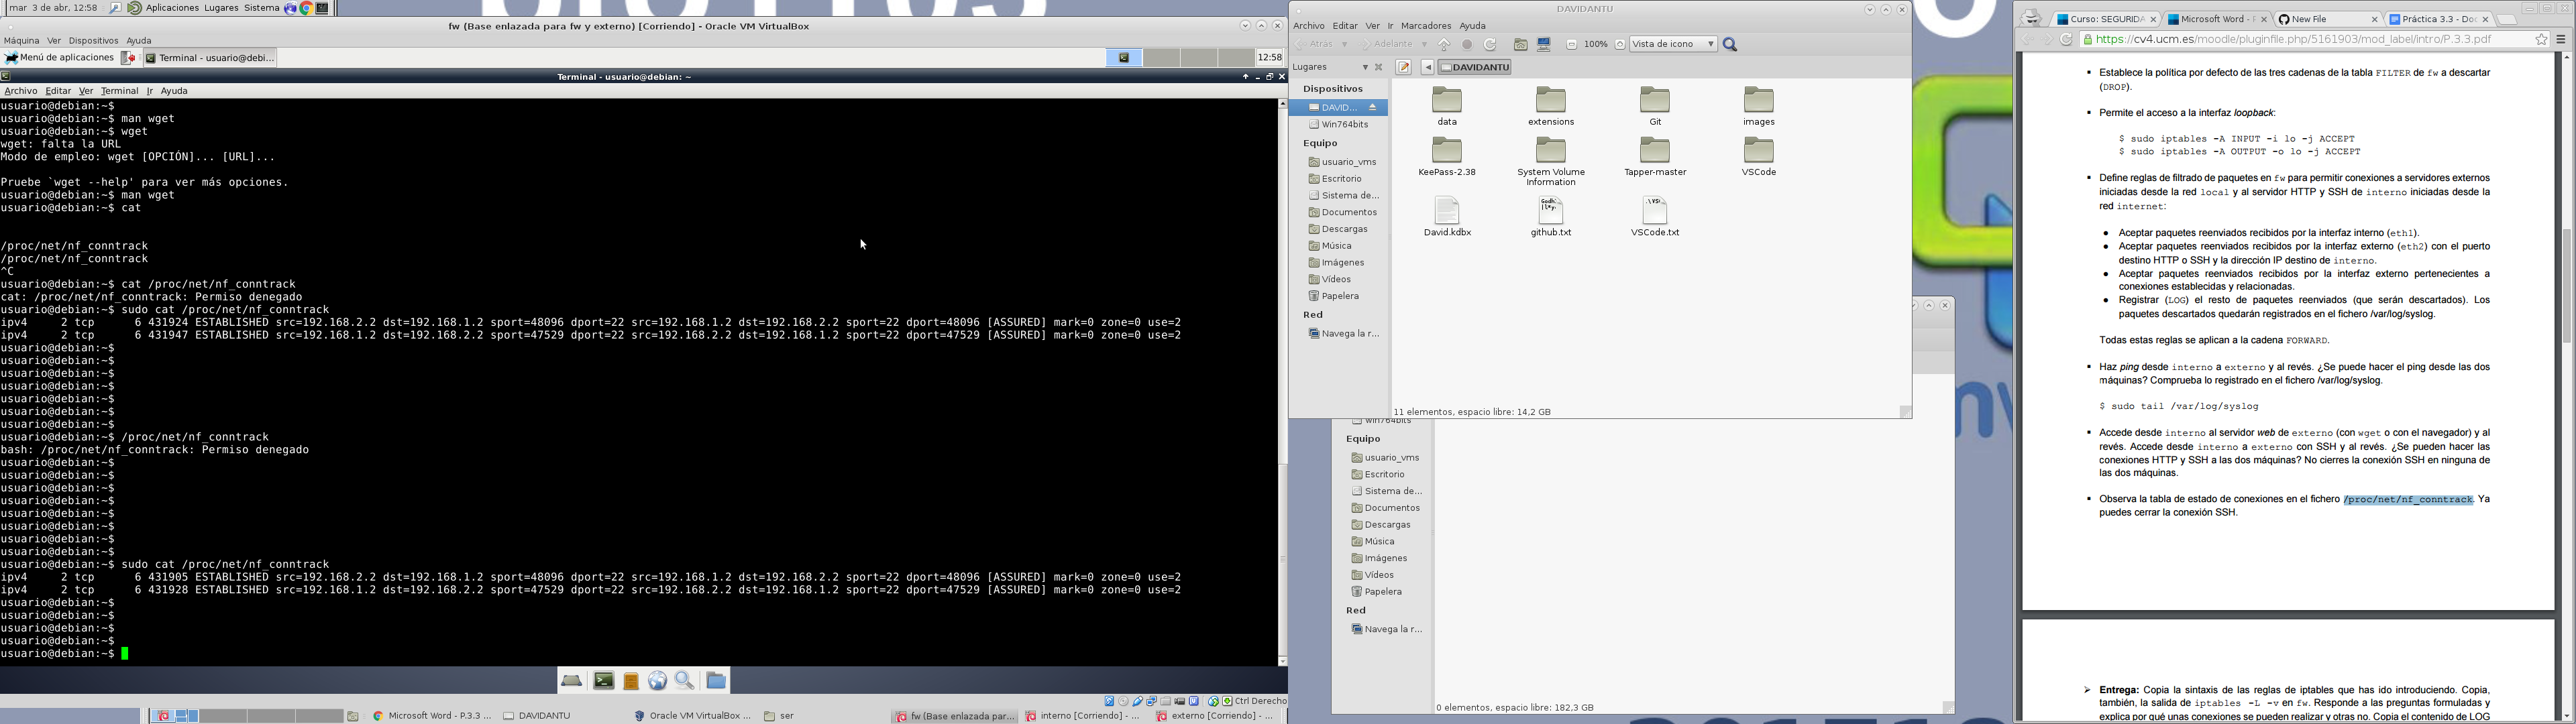
\includegraphics[width = \textwidth]{ssh}
        \caption{Estado de las conexiones.}
      \end{figure}

      \begin{figure}[H]
        \centering
        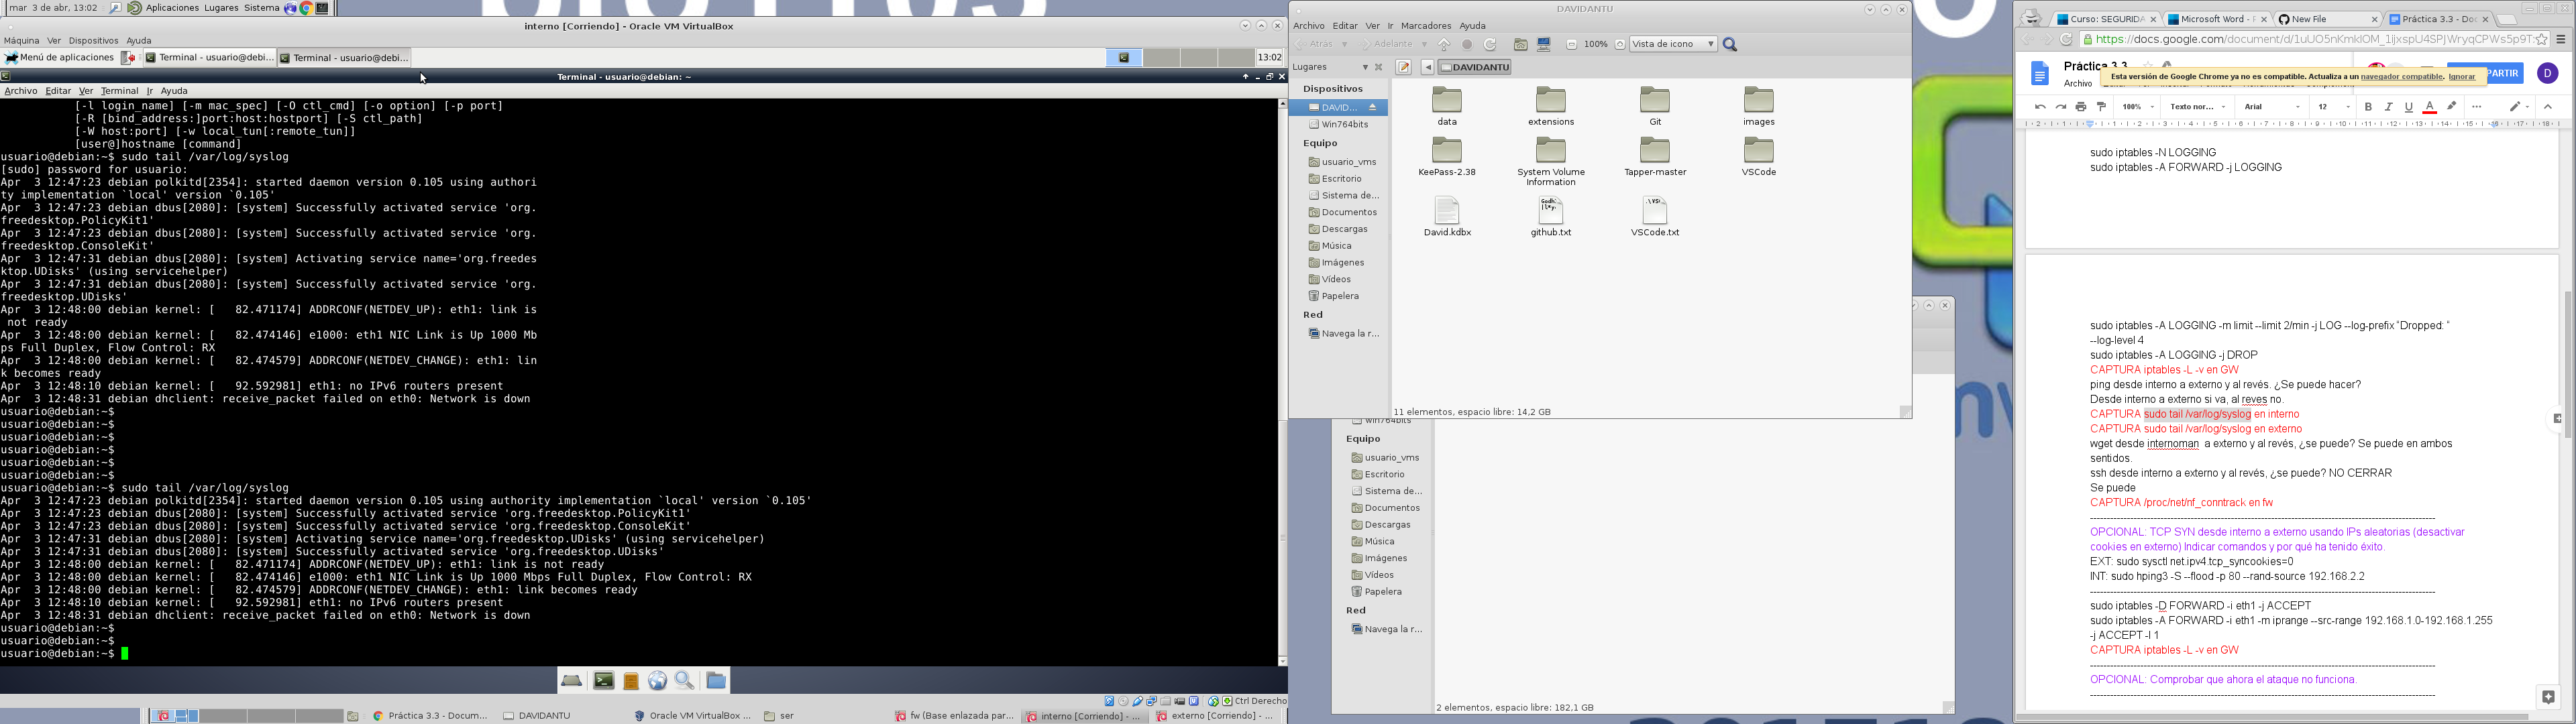
\includegraphics[width = \textwidth]{loginterno}
        \caption{Log de la máquina interna.}
      \end{figure}

      \begin{figure}[H]
        \centering
        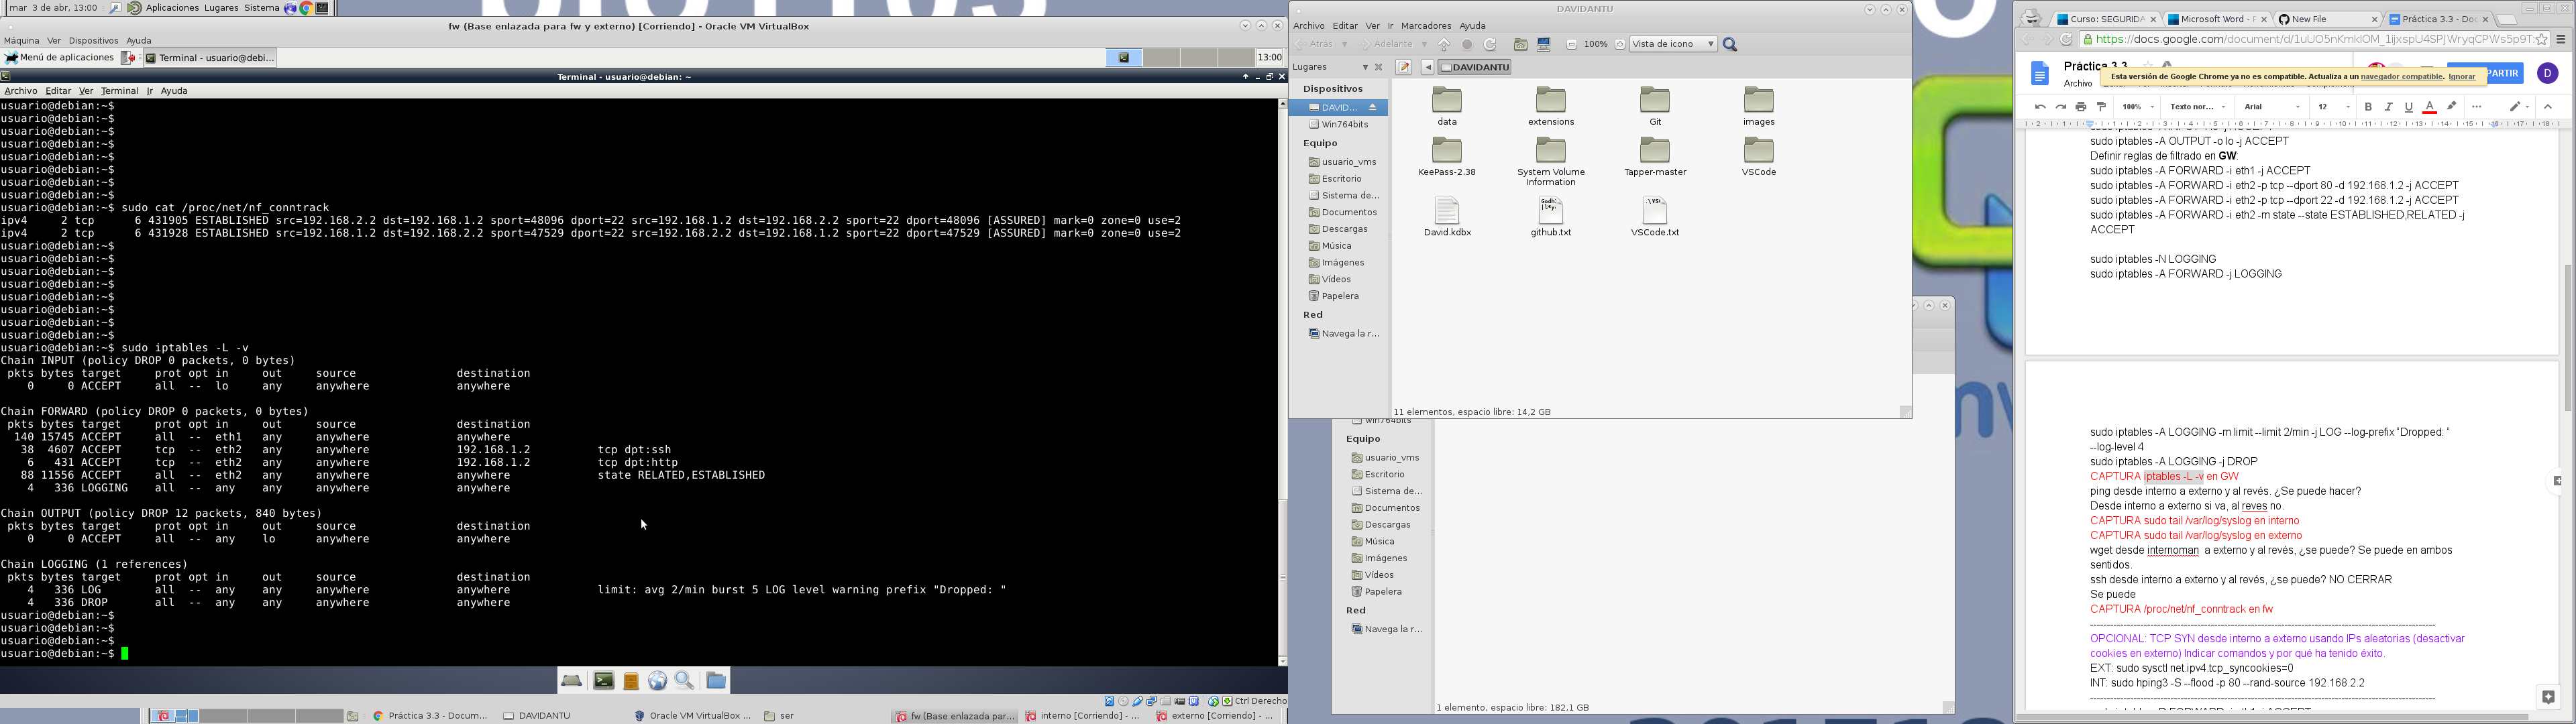
\includegraphics[width = \textwidth]{iptables}
        \caption{IP tables.}
      \end{figure}

      \begin{figure}[H]
        \centering
        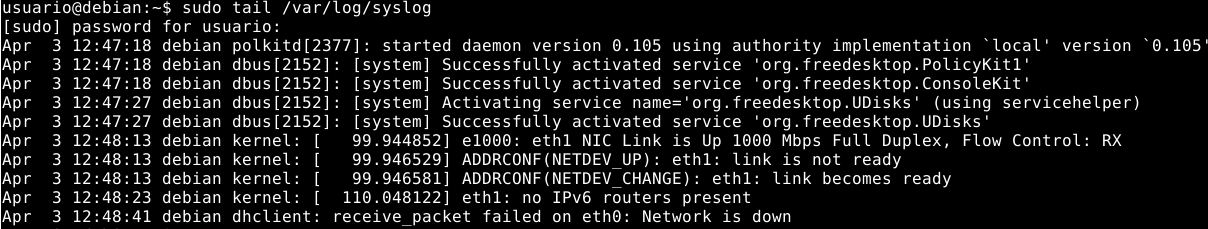
\includegraphics[width = \textwidth]{logexterno}
        \caption{Log de la maquina externa.}
      \end{figure}

    \subsection{Prevención del ataque}
      \par
      Elimina la primera regla de la cadena FORWARD y añade otra regla que
      acepte paquetes reenviados recibidos por la interfaz interno, pero solo de
      direcciones origen pertenecientes a la red local (192.168.1.0/24).
      Insertar esta regla en la posición 1 de la cadena (usar opción –I).\\
      \vspace{2mm}
      sudo iptables -D FORWARD -i eth1 -j ACCEPT\\
      sudo iptables -I FORWARD 1 -i eth1 -m iprange --src-range
        192.168.1.0-192.168.1.255  -j ACCEPT

      \begin{figure}[H]
        \centering
        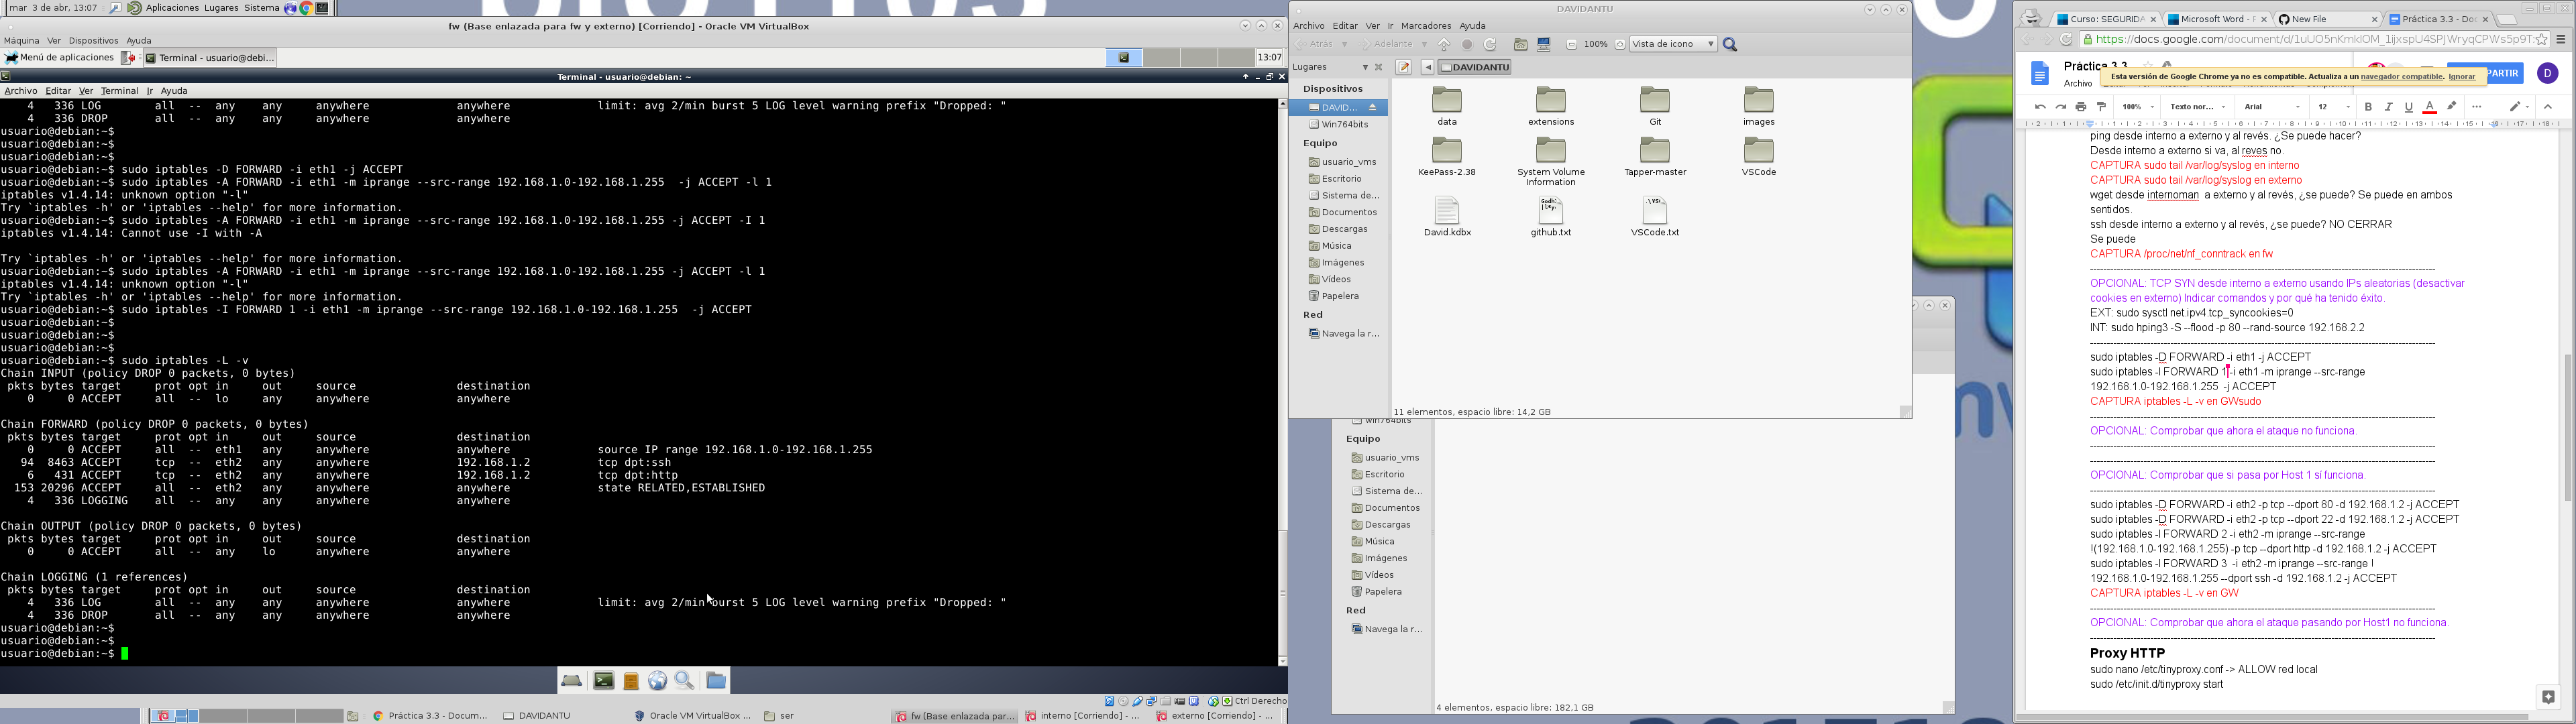
\includegraphics[width = \textwidth]{iptables2}
        \caption{IP tables.}
      \end{figure}

      \bigskip
      \par
      Elimina las reglas de la cadena FORWARD que permiten el paso de paquetes
      HTTP y SSH por eth2 y añade otras que acepten paquetes reenviados
      recibidos por la interfaz externo con puerto destino HTTP o SSH, dirección
      IP destino de interno y direcciones origen distintas a las de la red local
      (usa el operador negación !). Insertarlas en las posiciones 2 y 3 de la
      cadena (usar opción –I).\\
      \vspace{2mm}
      sudo iptables -D FORWARD -i eth2 -p tcp --dport 80 -d 192.168.1.2 -j
        ACCEPT\\
      sudo iptables -D FORWARD -i eth2 -p tcp --dport 22 -d 192.168.1.2 -j
        ACCEPT\\
      sudo iptables -I FORWARD 2 -i eth2 ! -s  192.168.1.0/24 -p tcp --dport
        http -d 192.168.1.2 -j ACCEPT\\
      sudo iptables -I FORWARD 3 -i eth2 ! -s  192.168.1.0/24 -p tcp --dport ssh
        -d 192.168.1.2 -j ACCEPT

      \begin{figure}[H]
        \centering
        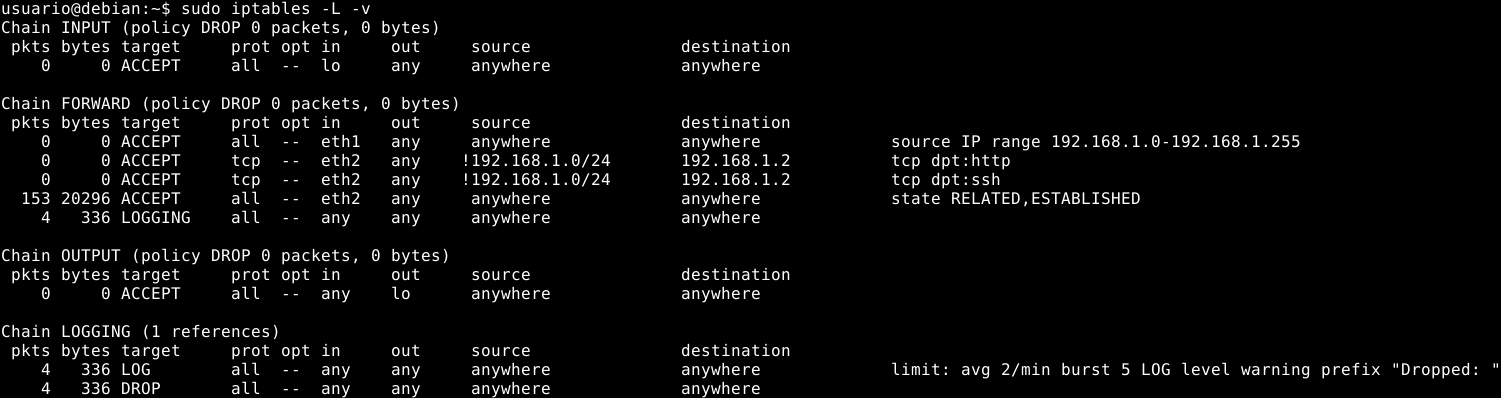
\includegraphics[width = \textwidth]{iptables3}
        \caption{IP tables.}
      \end{figure}

  \section{ProxyHTTP}
    \par
    Aceptar paquetes entrantes recibidos por la interfaz interno con puerto
    destino 8888 (donde escucha el proxy).\\
    \vspace{2mm}
    sudo iptables -A INPUT -i eth1 -p tcp --dport 8888 -j ACCEPT

    \bigskip
    \par
    Aceptar paquetes salientes enviados por la interfaz externo con puerto
    destino HTTP.\\
    \vspace{2mm}
    sudo iptables -A OUTPUT -p tcp --dport http -j ACCEPT

    \bigskip
    \par
    Aceptar paquetes entrantes de conexiones establecidas.\\
    \vspace{2mm}
    sudo iptables -A INPUT -i eth1 -m state --state ESTABLISHED -j ACCEPT

    \bigskip
    \par
    Aceptar paquetes salientes de conexiones establecidas.\\
    \vspace{2mm}
    sudo iptables -A OUTPUT -m state --state ESTABLISHED -j ACCEPT

    \bigskip
    \par
    Descartar paquetes reenviados recibidos por la interfaz eth1 con puerto
    destino HTTP.\\
    \vspace{2mm}
    sudo iptables -I FORWARD 1 -i eth1 -p tcp --dport http -j DROP

    \begin{figure}[H]
      \centering
      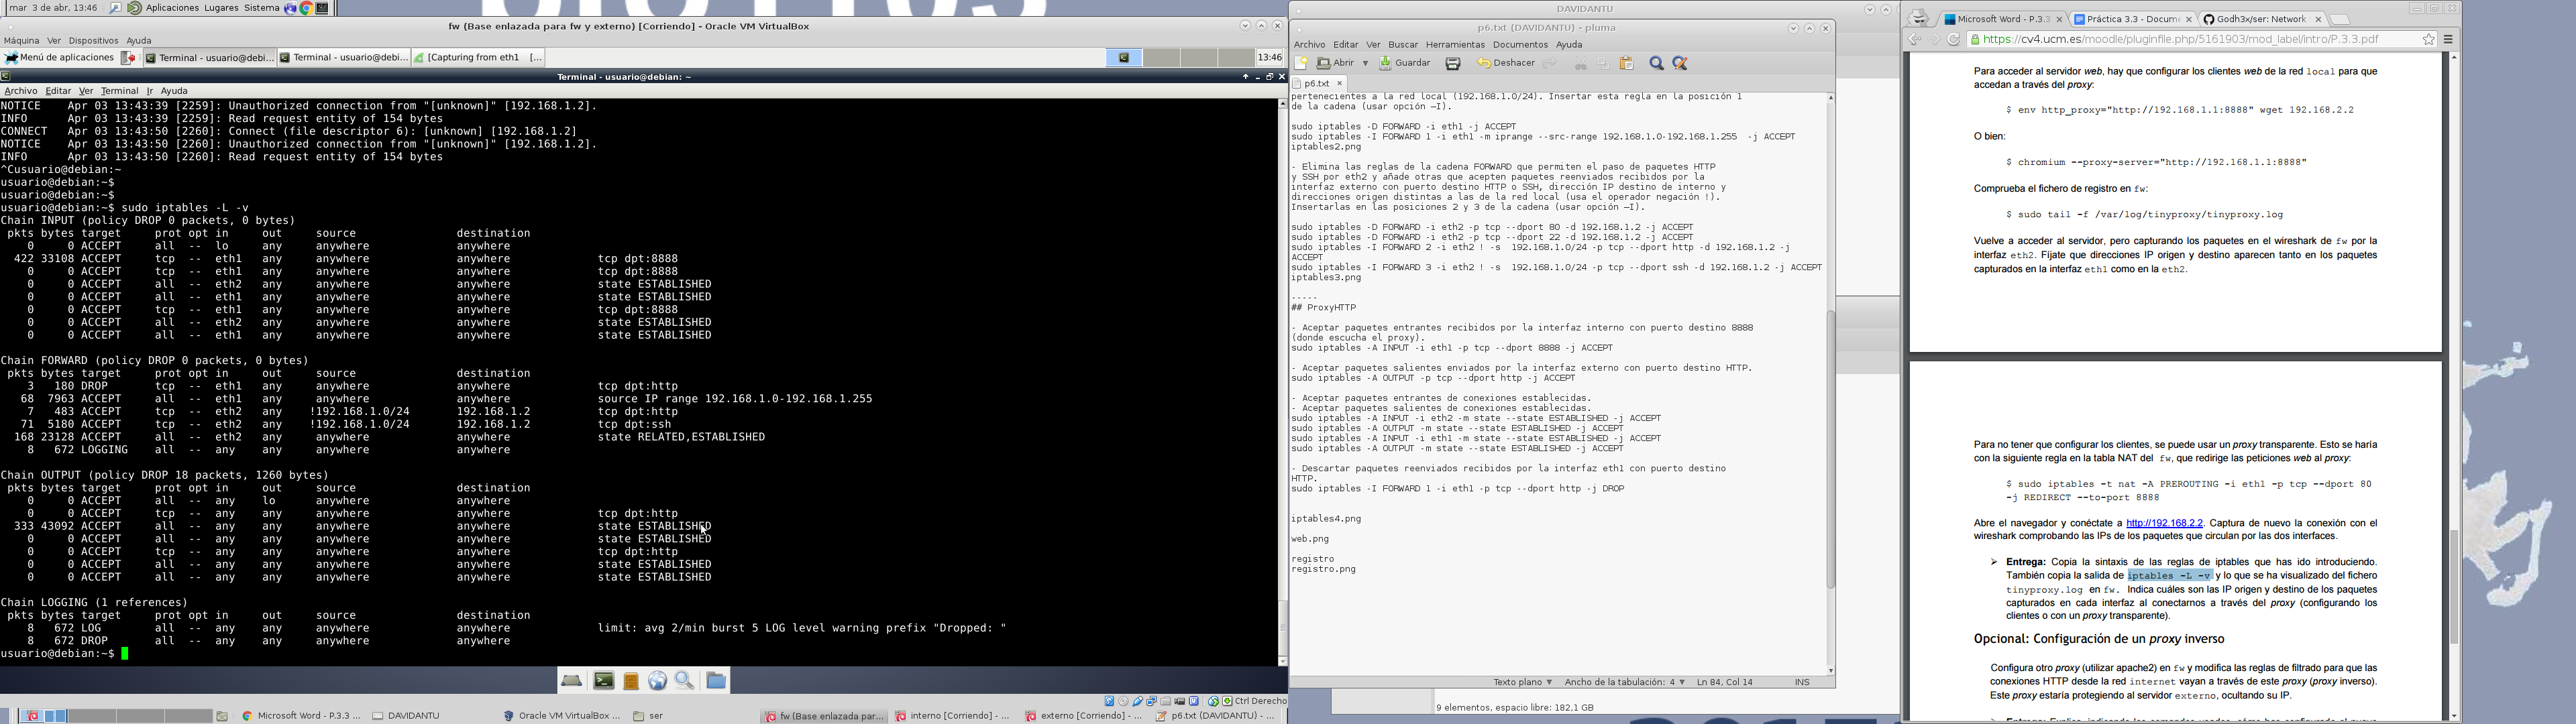
\includegraphics[width = \textwidth]{iptables4}
      \caption{IP tables.}
    \end{figure}

    \begin{figure}[H]
      \centering
      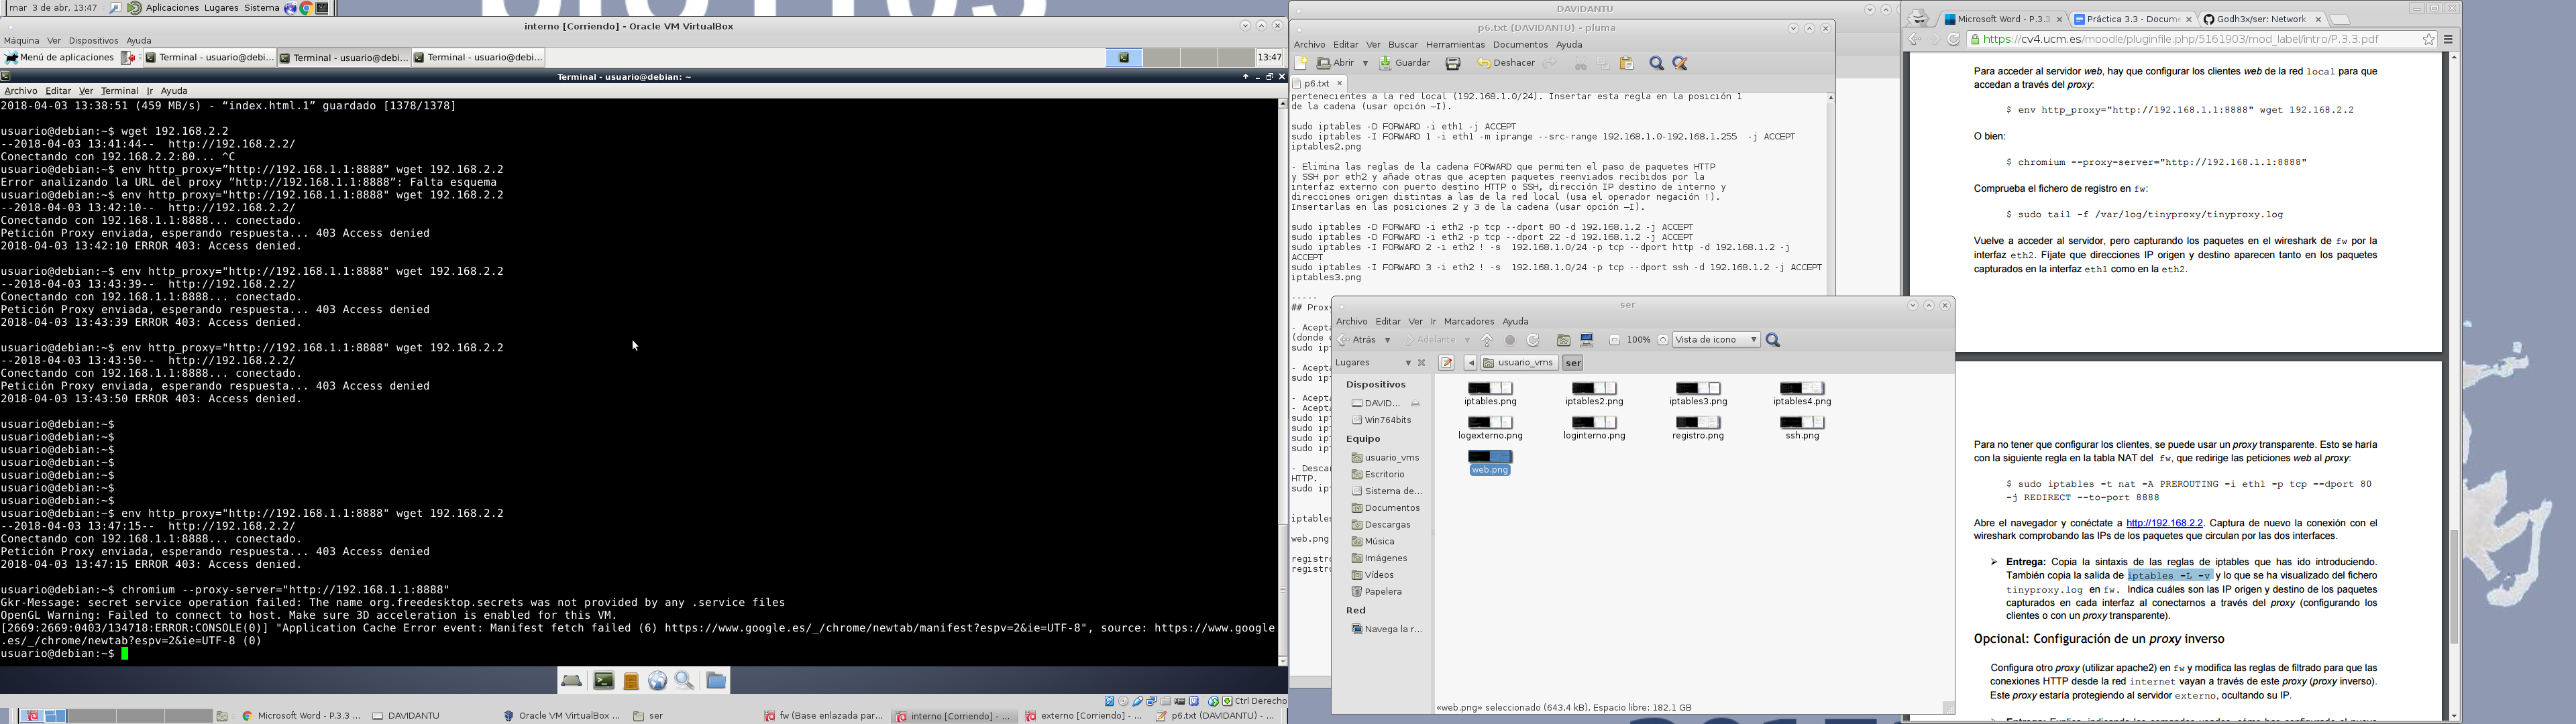
\includegraphics[width = \textwidth]{web}
      \caption{Conexión al servidor web.}
    \end{figure}

    \begin{figure}[H]
      \centering
      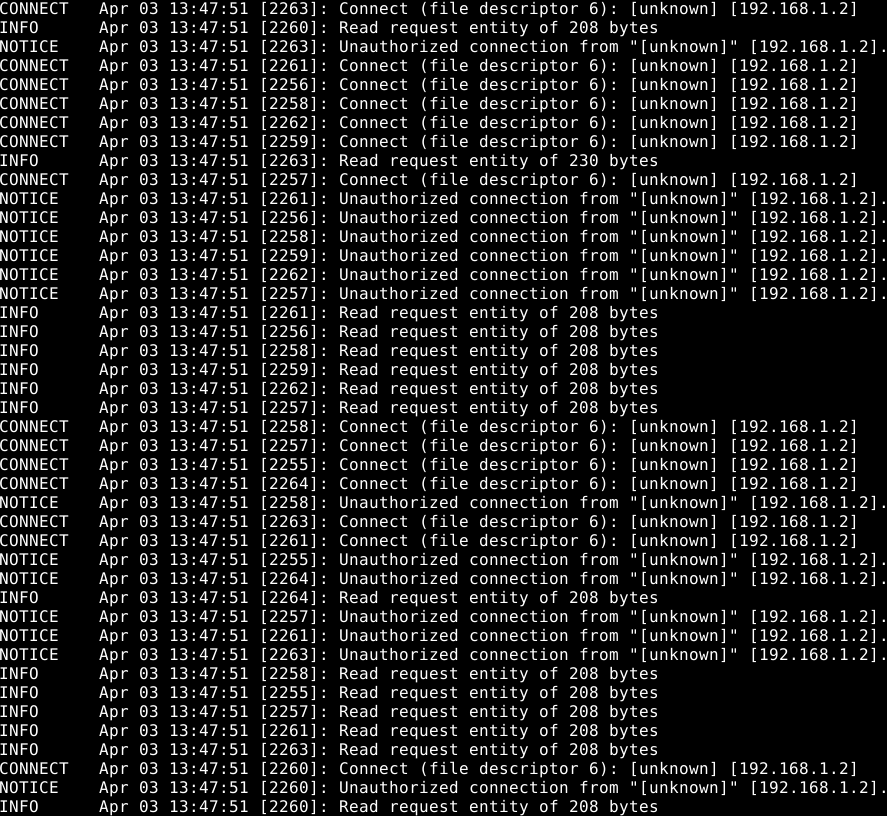
\includegraphics[width = \textwidth]{registro}
      \caption{Fichero de registro del router.}
    \end{figure}

    \bigskip
    \par
    No hemos averiguado que regla tenemos mal pero sabemos que al menos una lo
    está porque la conexión al servidor se rechaza, lo cual está bien, pero la
    que se hace mediante el proxy también, y no debería.
\end{document}
